\documentclass[12pt]{exam}

\usepackage[margin=0.5in]{geometry}
\usepackage{amsmath,amssymb}
\usepackage{tikz,soul}
\usepackage{diagbox}
\usetikzlibrary{arrows,automata,positioning}

\newcommand{\ds}{\displaystyle}
\newcommand{\bs}{\backslash}
\newcommand{\on}{\operatorname}
\newcommand{\R}{\mathbb{R}}
\newcommand{\Z}{\mathbb{Z}}
\newcommand{\N}{\mathbb{N}}

\begin{document}
\pagestyle{empty}
\subsubsection*{Homework 6 - Computer Science 461 \hfill Name: \underline{\hspace*{2in}}}

\textit{Due Monday, March 3.} % You can e-mail your code for the computer programming problems to me at }\verb|blins@hsc.edu|.

\begin{questions}

\question Construct a context free grammar that generates each of the following languages.
\begin{parts}
\part $\{a^{2n} b^n : n \in \N\}$
\begin{solution}
\begin{align*}
S &\rightarrow aaSb \\
S &\rightarrow \epsilon 
\end{align*}
\end{solution}
\vfill

\part $\{w \in \{0,1\}^* : w \text{ starts and ends with the same symbol.}\}$
\begin{solution}
\begin{align*}
S &\rightarrow 0R0 \\
S &\rightarrow 1R1 \\
R &\rightarrow R1 \\
R &\rightarrow R0 \\
R &\rightarrow \epsilon
\end{align*}
\end{solution}
\vfill

\part $\{w \in \{a,b,c\}^* : \text{ length of } w \text{ is odd and its middle symbol is }b\}$ 
\begin{solution}
\begin{align*}
S &\rightarrow M \\
M &\rightarrow LML \\
L &\rightarrow a \\
L &\rightarrow b \\
L &\rightarrow c \\
M &\rightarrow b \\
\end{align*}
\end{solution}
\vfill


\part $\{w \in \{0,1\}^* : w \text{ is a palindrome.}\}$ Hint: \textit{Make sure your grammar generates both even and odd length palindromes.}
\begin{solution}
\begin{align*}
S &\rightarrow 0S0 \\
S &\rightarrow 1S1 \\
S &\rightarrow 0 \\
S &\rightarrow 1 \\
S &\rightarrow \epsilon \\
\end{align*}
\end{solution}
\vfill
\end{parts}

\question Identify the parts of the tuple $(V, \Sigma, R, S)$ in your answer to problem 1 part (b).  
\begin{solution}
$$V = \{S,R\}, \Sigma = \{0,1\}, R = \{S \rightarrow 0R0, S \rightarrow 1R1, R \rightarrow R1, R \rightarrow R0, R \rightarrow \epsilon \}, \text{ and } S = S.$$
\end{solution}
\vfill

\newpage
\question Let $\Sigma = \{ \verb|(,),[,]| \}$. That is, $\Sigma$ is the alphabet consisting of the four symbols \verb|(|, \verb|)|, \verb|[|, and \verb|]|. Let $L$ be the language over $\Sigma$ consisting of strings in which both parentheses and brackets are balanced. For example, the string \verb|([][()()])([])| is in $L$ but \verb|[(])| is not. Find a context-free grammar that generates the language $L$.
\vfill
\question Draw two different parse trees for the string $ababbaab$ to show that the following grammar is ambiguous.

\begin{minipage}{1.5in}
\begin{align*}
S &\rightarrow SS \\
S &\rightarrow aSb \\
S &\rightarrow bSa \\
S &\rightarrow \epsilon 
\end{align*}
\end{minipage}
\vfill

\question Suppose that the string $abbcabac$ has the following parse tree, according to some grammar $G$. Identify 5 production rules that must be rules in the grammar $G$.  
\begin{flushright}
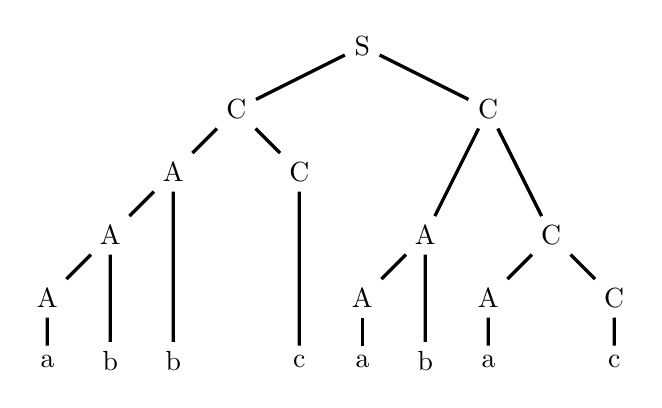
\begin{tikzpicture}[scale=0.8]
\path (0,10) node (A) {S};
\path (-2,9) node (B1) {C};
\path (2,9)  node (B2) {C};
\path (-3,8) node (C1) {A};
\path (-1,8) node (C2) {C};
\path (-4,7) node (D1) {A};
\path (1,7) node (D2) {A};
\path (3,7) node (D3) {C};
\path (-5,6) node (E1) {A};
\path (0,6) node (E2) {A};
\path (2,6) node (E3) {A};
\path (4,6) node (E4) {C};
\path (-5,5) node (F1) {a};
\path (-4,5) node (F2) {b};
\path (-3,5) node (F3) {b};
\path (-1,5) node (F4) {c};
\path (0,5) node (F5) {a};
\path (1,5) node (F6) {b};
\path (2,5) node (F7) {a};
\path (4,5) node (F8) {c};

\draw[very thick] (A) to (B1);
\draw[very thick] (A) to (B2);
\draw[very thick] (B1) to (C1);
\draw[very thick] (B1) to (C2);
\draw[very thick] (B2) to (D2);
\draw[very thick] (B2) to (D3);
\draw[very thick] (C1) to (D1);
\draw[very thick] (D1) to (E1);
\draw[very thick] (D2) to (E2);
\draw[very thick] (D3) to (E3);
\draw[very thick] (D3) to (E4);
\draw[very thick] (E1) to (F1);
\draw[very thick] (D1) to (F2);
\draw[very thick] (C1) to (F3);
\draw[very thick] (C2) to (F4);
\draw[very thick] (E2) to (F5);
\draw[very thick] (D2) to (F6);
\draw[very thick] (E3) to (F7);
\draw[very thick] (E4) to (F8);

\end{tikzpicture}
\end{flushright}

\end{questions}
\end{document}
